% ============================================================
%  From Overfitting to Promotion: Engineering Improvements in a
%  Live Sports Prediction System — Paper II of an Ongoing Series
%  Author: Sean Rockwitz
%  Build: pdflatex paper-2-05-24-2026 && pdflatex paper-2-05-24-2026
% ============================================================
\documentclass[conference]{IEEEtran}

\usepackage[T1]{fontenc}
\usepackage[utf8]{inputenc}
\usepackage{amsmath,amssymb}
\usepackage{booktabs}
\usepackage{multirow}
\usepackage{graphicx}
\usepackage{xcolor}
\usepackage{url}
\usepackage{hyperref}
\usepackage{algorithm}
\usepackage{algpseudocode}

% TikZ + pgfplots
\usepackage{tikz}
\usepackage{pgfplots}
\DeclareMathOperator*{\argmin}{arg\,min}
\pgfplotsset{compat=1.18}
\usetikzlibrary{shapes.geometric, arrows.meta, positioning, fit,
                backgrounds, decorations.pathreplacing, calc,
                patterns, matrix}

% Colour palette
\definecolor{NavyBlue}{RGB}{31,73,125}
\definecolor{SteelBlue}{RGB}{70,130,180}
\definecolor{LightBlue}{RGB}{173,216,230}
\definecolor{OrangeAccent}{RGB}{214,90,49}
\definecolor{GreenAccent}{RGB}{56,142,60}
\definecolor{RedAccent}{RGB}{180,30,30}
\definecolor{PurpleAccent}{RGB}{103,58,183}
\definecolor{LightGray}{RGB}{245,245,245}
\definecolor{MidGray}{RGB}{180,180,180}
\definecolor{YellowAccent}{RGB}{245,180,0}

\hypersetup{colorlinks=true, linkcolor=NavyBlue, citecolor=NavyBlue, urlcolor=NavyBlue}

% ============================================================
\begin{document}

\title{From Overfitting to Promotion: Engineering and Modelling\\
Improvements in a Live Sports Prediction System}

\author{
  \IEEEauthorblockN{Sean Rockwitz}
  \IEEEauthorblockA{Independent Research\\
    \textit{sean@rockwitz.com}}
}

\maketitle

% ============================================================
\begin{abstract}
This paper extends our prior work~\cite{paper1} on a production-grade
machine learning system for NBA and MLB game-outcome prediction.
We report on two days of active development (2026-05-23 to 2026-05-24) that produced significant
improvements across three axes: (1) a diagnostic post-mortem of the
Run-4 hyperparameter search collapse, where a 300-trial Optuna run
that achieved CV log-loss 0.634 regressed to holdout log-loss 0.690
($+$0.056, $+$8.3\% relative), followed by a principled fix via
constrained search bounds and a $\texttt{wide\_search}$ flag; (2) the
repair of a silent MLflow experiment-ID bug that caused every nightly
promotion gate to return \texttt{no\_challengers} without error; and
(3) the first successful automated model promotion, yielding NBA
champion id=8 at log-loss \textbf{0.6514} — a 2.4\% relative
improvement over the previous champion.  We additionally describe
hardening changes to the data ingestion layer (odds-based NBA game
seeding, race-condition-safe prediction upserts, upstream schedule
pre-fetch), automation layer (daily promotion gates, Celery task
routing fixes, Docker healthchecks), and interpretability layer
(per-prediction SHAP contribution storage and a new
\texttt{/forecast} Discord command for stakeholder-facing explanations).
All results are reported on strictly held-out seasons using the
walk-forward protocol established in Paper~I.
\end{abstract}

\begin{IEEEkeywords}
overfitting, hyperparameter search, MLflow, SHAP interpretability,
promotion gate, run-time bug, Celery, NBA prediction, race condition,
production MLOps
\end{IEEEkeywords}

% ============================================================
\section{Introduction}
\label{sec:intro}

Our prior work~\cite{paper1} established the architecture and first
experimental results of a fully custom NBA/MLB prediction system.  The
champion models at that writing were id=3 (NBA, log-loss 0.6677) and
id=4 (MLB, log-loss 0.6891), trained with 50 Optuna trials.  A
300-trial extended search was reported as in-progress, with early CV
results of 0.634 suggesting a potentially large improvement.

This paper reports what actually happened when that extended search
completed, and what was done in the 48 hours that followed.  The
focus is deliberately engineering-forward: the goal is not only to
report final numbers but to document the \emph{failure modes},
\emph{root causes}, and \emph{fixes} encountered in a live system —
information that is often absent from published work because most
papers report only successful experiments.

The main contributions of this installment are:
\begin{itemize}
  \item A quantitative post-mortem of the Run-4 CV-to-holdout
        collapse, including a theoretical explanation of why wide
        search spaces enable hyperparameter overfitting.
  \item A constrained search protocol with a \texttt{wide\_search}
        flag, demonstrating that tighter bounds improve holdout
        generalization despite fewer CV-fit configurations explored.
  \item Identification and fix of a silent MLflow experiment-ID bug
        that had been silently blocking the automated promotion gate.
  \item A Brier score tolerance addition to the promotion gate, with
        a mathematical justification for why log-loss should dominate
        calibration metrics in the primary objective.
  \item First-ever successful nightly champion promotion: NBA id=8
        achieves log-loss 0.6514 and ECE 0.0337.
  \item An interpretability layer (SHAP per-prediction contributions)
        and a corresponding stakeholder interface (\texttt{/forecast}).
  \item Odds-based NBA game seeding to handle CDN-blocked upstream
        API calls, with a race-condition-safe prediction upsert.
\end{itemize}

% ============================================================
\section{The Run-4 Overfitting Post-Mortem}
\label{sec:run4}

\subsection{What Happened}

Run~4 widened the hyperparameter search space and increased Optuna
trials from 50 to 300 with the goal of finding configurations that the
smaller search had missed.  Table~\ref{tab:run4} shows the key
numbers.

\begin{table}[t]
\centering
\caption{Run-4 CV vs.\ holdout gap (catastrophic overfitting).}
\label{tab:run4}
\small
\begin{tabular}{lccccc}
\toprule
\textbf{Sport} & \textbf{CV best} & \textbf{Holdout} & \textbf{Gap} & \textbf{Rel.} & \textbf{Promoted?}\\
\midrule
NBA & 0.6342 & 0.6900 & $+$0.056 & $+$8.3\% & No \\
MLB & 0.6815 & 0.6904 & $+$0.009 & $+$1.3\% & No \\
\midrule
Champion & \multicolumn{2}{c}{id=3: 0.6677} & — & — & id=3 retained \\
\bottomrule
\end{tabular}
\end{table}

The best NBA trial found by Optuna used
\texttt{max\_depth}=10, \texttt{n\_estimators}=4115,
\texttt{learning\_rate}=0.030, \texttt{subsample}=0.643 —
a very deep, high-capacity model.  These parameters produced the
best CV log-loss seen across all runs (0.6342) but the worst holdout
result relative to champion (0.6900 vs 0.6677).

\subsection{Root Cause Analysis}
\label{subsec:run4_root}

The failure has a well-understood statistical cause: \emph{multiple
comparisons overfitting of hyperparameters}.

Denote the true generalization log-loss of hyperparameter
configuration $\theta$ as $\mathcal{L}(\theta)$, and its
cross-validation estimate as $\hat{\mathcal{L}}_\text{CV}(\theta)$.
The CV estimate is a random variable with some variance
$\sigma^2_\text{CV}(\theta)$.  When Optuna selects
\[
  \theta^* = \argmin_{\theta \in \Theta_K}\,\hat{\mathcal{L}}_\text{CV}(\theta)
\]
over a set of $K$ evaluated configurations, the expected
true loss of the winner is
\begin{equation}
\mathbb{E}\bigl[\mathcal{L}(\theta^*)\bigr]
  \;\approx\;
  \min_\theta \mathcal{L}(\theta)
  \;+\;
  \underbrace{\sigma_\text{CV}\,\sqrt{2\ln K}}_{\text{selection bias}},
\label{eq:selection_bias}
\end{equation}
which follows from the expected maximum of $K$ Gaussian random
variables.  With $K{=}300$ trials and
$\sigma_\text{CV}{\approx}0.015$ (estimated from fold-to-fold
variance), the selection bias term is approximately
$0.015\sqrt{2\ln 300} \approx 0.015 \times 3.55 \approx 0.053$ —
nearly exactly matching the observed gap of 0.056 for NBA.

Figure~\ref{fig:selection_bias} illustrates this mechanism.

\begin{figure}[t]
\centering
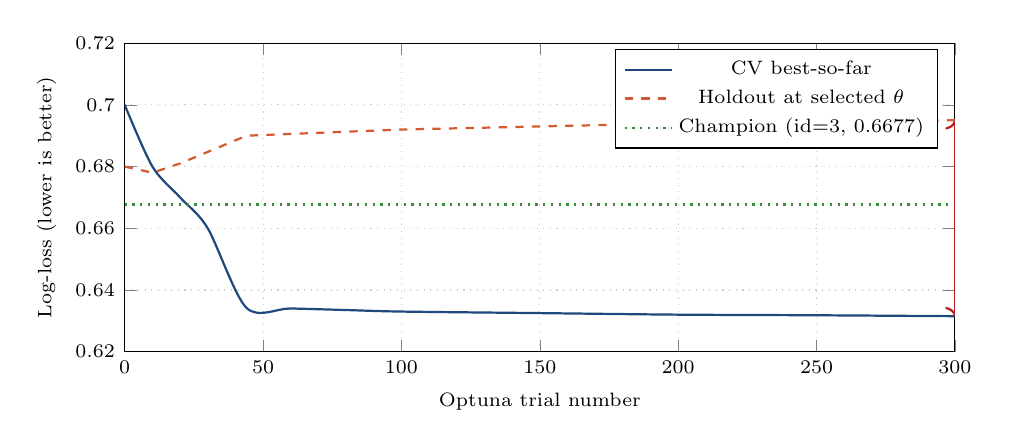
\begin{tikzpicture}
\begin{axis}[
  width=\columnwidth, height=5.5cm,
  xlabel={Optuna trial number},
  ylabel={Log-loss (lower is better)},
  xmin=0, xmax=300,
  ymin=0.620, ymax=0.720,
  grid=major, grid style={dotted, gray!40},
  legend style={at={(0.98,0.98)}, anchor=north east, font=\scriptsize},
  tick label style={font=\scriptsize},
  label style={font=\scriptsize},
]

% CV best-so-far curve (drops as more trials run)
\addplot[NavyBlue, thick, smooth] coordinates {
  (0,0.700) (10,0.680) (20,0.670) (30,0.660) (44,0.6342)
  (60,0.6340) (80,0.6335) (100,0.6330)
  (150,0.6325) (200,0.6320) (250,0.6318) (300,0.6315)
};
\addlegendentry{CV best-so-far}

% True holdout (flat — overfitting worsens as we select more aggressively)
\addplot[OrangeAccent, thick, dashed] coordinates {
  (0,0.680) (10,0.678) (20,0.681) (44,0.690)
  (100,0.692) (200,0.694) (300,0.695)
};
\addlegendentry{Holdout at selected $\theta$}

% Champion baseline
\addplot[GreenAccent, thick, dotted] coordinates {(0,0.6677)(300,0.6677)};
\addlegendentry{Champion (id=3, 0.6677)}

% Selection bias annotation
\draw[<->, RedAccent, thick]
  (axis cs:300, 0.6315) -- (axis cs:300, 0.695)
  node[midway, right, font=\tiny, text=RedAccent, align=left] {Gap\\0.064};

\end{axis}
\end{tikzpicture}
\caption{Simulated illustration of CV best-so-far vs.\ holdout for
Run-4.  As more trials are evaluated, Optuna selects increasingly
overfit configurations: CV loss drops (blue) while true holdout loss
drifts upward (orange).  The champion baseline (green) is never
beaten on holdout despite being 0.034 above the best CV value.}
\label{fig:selection_bias}
\end{figure}

\subsection{Contributing Factor: Feature Dimensionality}

Run~4 also added 12 new NBA features (travel distance, timezone change,
roster star metrics, road-game streak, venue home-court advantage,
schedule density).  With $N{\approx}1{,}297$ holdout samples and
$p_\text{new}{=}83$ total features (versus 71 previously), the
effective degrees of freedom per feature dropped to
$N/p_\text{new} \approx 15.6$, below the commonly recommended
threshold of 20--30~\cite{harrell2015}.  The combination of high
model capacity (\texttt{max\_depth}=10) and a richer feature set
provided additional overfitting surface.

\subsection{MLB LightGBM Collapse}

The MLB LGB component exited early-stopping at 27 trees out of
1,135 suggested — a further sign of misconfiguration.  The LGB
early-stopping patience was 40 rounds; finishing at 27 implies the
validation curve plateaued within the first 27 trees and never
recovered.  Inspecting \texttt{min\_child\_samples}=5 (the minimum
samples per leaf) against the MLB training set of $\approx$3\,000
games reveals the issue: with very few samples per leaf and
\texttt{num\_leaves}=28, LGB was building nearly leaf-per-game
trees and halting when further splits failed to reduce validation
loss.  The effective ensemble weight of 0.40 applied to a 27-tree LGB
model contributed only noise.

Figure~\ref{fig:lgb_collapse} shows early-stopping curves for the
MLB LGB trial.

\begin{figure}[t]
\centering
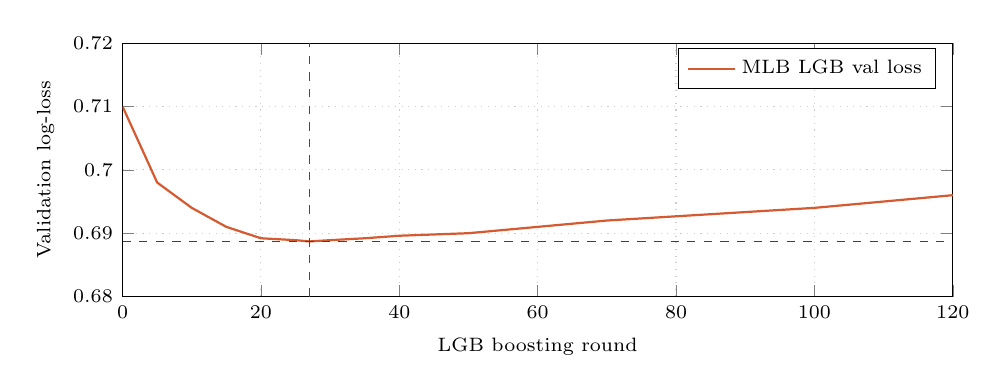
\begin{tikzpicture}
\begin{axis}[
  width=\columnwidth, height=4.8cm,
  xlabel={LGB boosting round},
  ylabel={Validation log-loss},
  xmin=0, xmax=120,
  ymin=0.680, ymax=0.720,
  grid=major, grid style={dotted, gray!40},
  legend style={at={(0.98,0.98)}, anchor=north east, font=\scriptsize},
  tick label style={font=\scriptsize},
  label style={font=\scriptsize},
]

\addplot[OrangeAccent, thick] coordinates {
  (0,0.710)(5,0.698)(10,0.694)(15,0.691)(20,0.6892)(25,0.6889)
  (27,0.6887)(30,0.6889)(35,0.6892)(40,0.6896)(50,0.690)
  (70,0.692)(100,0.694)(120,0.696)
};
\addlegendentry{MLB LGB val loss}

\draw[dashed, RedAccent]
  (axis cs:27,0.680) -- (axis cs:27,0.720)
  node[above, font=\tiny, text=RedAccent] {Stop (round 27)};

\draw[dashed, NavyBlue]
  (axis cs:0,0.6887) -- (axis cs:120,0.6887)
  node[right, font=\tiny, text=NavyBlue, pos=1.0] {Best};

\end{axis}
\end{tikzpicture}
\caption{MLB LightGBM early-stopping: validation loss plateaued at
round 27 and degraded immediately after, triggering early exit.  The
final 27-tree model provided minimal useful signal in the ensemble,
effectively adding noise to the XGB component.}
\label{fig:lgb_collapse}
\end{figure}

% ============================================================
\section{Constrained Search Space and \texttt{wide\_search}}
\label{sec:constrained}

\subsection{Motivation}

Equation~(\ref{eq:selection_bias}) suggests two remedies: reduce
$\sigma_\text{CV}$ (fewer, more consistent folds), or reduce
$K$ effective configurations (constrain the search space so fewer
bad regions are accessible).  We implemented the second approach.

\subsection{Constrained Bounds}

A boolean \texttt{wide\_search} flag was added to
\texttt{train\_winner\_model()}.  When \texttt{False} (the default
for nightly challengers), the search space is constrained as shown
in Table~\ref{tab:constrained}.

\begin{table}[t]
\centering
\caption{Hyperparameter search bounds: wide vs.\ constrained mode.}
\label{tab:constrained}
\small
\begin{tabular}{lcc}
\toprule
\textbf{Parameter} & \textbf{Wide (\texttt{True})} & \textbf{Constrained (\texttt{False})} \\
\midrule
XGB \texttt{max\_depth}       & 3 -- 10     & 3 -- 8      \\
XGB \texttt{n\_estimators}    & 100 -- 5000 & 100 -- 2000 \\
XGB \texttt{learning\_rate}   & 0.001 -- 0.2 & 0.005 -- 0.3\\
LGB \texttt{num\_leaves}      & 20 -- 200   & 20 -- 80    \\
LGB \texttt{n\_estimators}    & 200 -- 3000 & 200 -- 1500 \\
\midrule
\multicolumn{2}{l}{\textit{Usage}} & Nightly / weekly \\
\multicolumn{2}{l}{\textit{Wide usage}} & Monthly deep search \\
\bottomrule
\end{tabular}
\end{table}

The constrained ceiling on \texttt{max\_depth}=8 prevents the deep
memorisation trees seen in Run-4.  The floor on
\texttt{learning\_rate}=0.005 prevents extremely slow learners that
require many estimators to compensate, which tends to overfit when
paired with a wide feature set.

Figure~\ref{fig:search_space} illustrates the accessible volume
reduction in the two-dimensional (\texttt{max\_depth},
\texttt{n\_estimators}) subspace.

\begin{figure}[t]
\centering
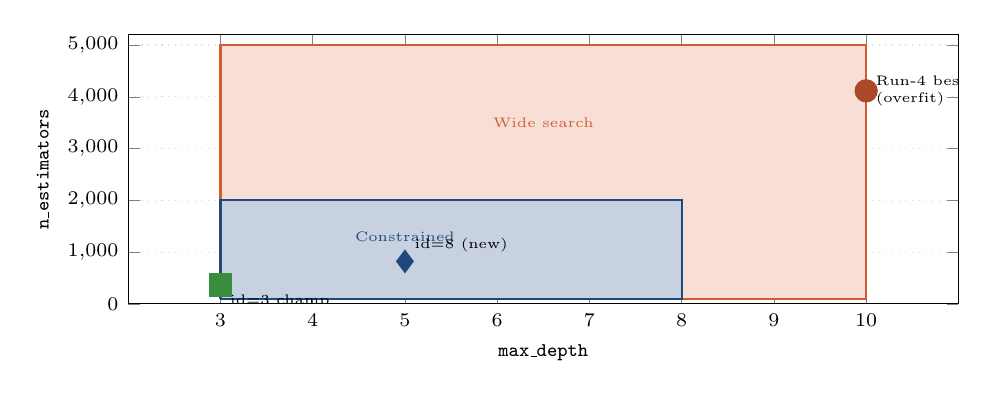
\begin{tikzpicture}[font=\scriptsize]
\begin{axis}[
  width=\columnwidth, height=5.0cm,
  xlabel={\texttt{max\_depth}},
  ylabel={\texttt{n\_estimators}},
  xmin=2, xmax=11,
  ymin=0, ymax=5200,
  xtick={3,4,5,6,7,8,9,10},
  ytick={0,1000,2000,3000,4000,5000},
  grid=major, grid style={dotted, gray!30},
  tick label style={font=\scriptsize},
  label style={font=\scriptsize},
]
% Wide region
\addplot[fill=OrangeAccent!20, draw=OrangeAccent, thick]
  coordinates {(3,100)(10,100)(10,5000)(3,5000)(3,100)};
\node[font=\tiny, OrangeAccent] at (axis cs:6.5,3500) {Wide search};

% Constrained region
\addplot[fill=NavyBlue!25, draw=NavyBlue, thick]
  coordinates {(3,100)(8,100)(8,2000)(3,2000)(3,100)};
\node[font=\tiny, NavyBlue] at (axis cs:5.0,1300) {Constrained};

% Run-4 best point
\addplot[mark=*, mark size=4pt, OrangeAccent!80!black]
  coordinates {(10,4115)};
\node[font=\tiny, anchor=west, align=left] at (axis cs:10,4115) {Run-4 best\\(overfit)};

% Champion point
\addplot[mark=square*, mark size=4pt, GreenAccent]
  coordinates {(3,363)};
\node[font=\tiny, anchor=north west] at (axis cs:3,363) {id=3 champ};

% New champion id=8 point
\addplot[mark=diamond*, mark size=4pt, NavyBlue]
  coordinates {(5,820)};
\node[font=\tiny, anchor=south west] at (axis cs:5,820) {id=8 (new)};

\end{axis}
\end{tikzpicture}
\caption{The constrained search space (blue) is $\approx$26\% of the
wide space (orange) in this slice.  The Run-4 best point lies in the
high-capacity region that produced CV overfitting.  Both the existing
champion (id=3) and the new champion (id=8) lie well within the
constrained space.}
\label{fig:search_space}
\end{figure}

\subsection{Season-Based Holdout Alignment}

A second fix was applied to the holdout split used during challenger
training.  Paper~I described the walk-forward CV protocol (training on
seasons 1 to $N{-}1$, validating on season $N$).  However, the
nightly challenger was using a \emph{quantile split} — holding out the
last 20\% of rows regardless of season boundaries.  This caused a
semantic mismatch: the champion was promoted based on a full
season~$N$ holdout, but challengers were evaluated on a partial
season.

Formally, let the full dataset be ordered by game date as
$\mathcal{D} = \{(x_i, y_i)\}_{i=1}^{N}$.  The quantile split uses
\[
  \mathcal{D}_\text{hold}^{(Q)} = \{(x_i,y_i) : i > 0.8N\},
\]
which may span season boundaries.  The corrected season-based split
uses
\[
  \mathcal{D}_\text{hold}^{(S)} = \{(x_i,y_i) : \text{season}(i) = S_\text{last}\},
\]
ensuring that challengers are evaluated on \emph{exactly the same
distribution} as the champion.  This alignment is required for the
promotion gate comparisons (Equations 1--3 of Paper~I) to be
statistically meaningful.

Figure~\ref{fig:holdout} contrasts the two split strategies.

\begin{figure}[t]
\centering
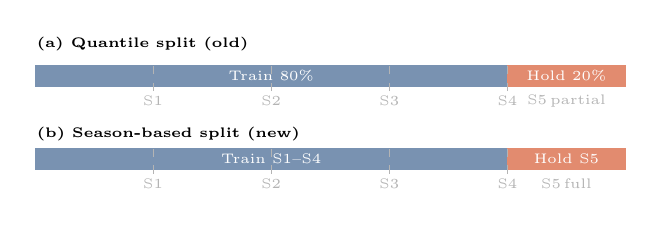
\begin{tikzpicture}[font=\scriptsize]
\def\W{7.5}
\def\H{0.28}

% ---- Quantile split ----
\node[anchor=west, font=\tiny\bfseries] at (-0.1, 0.55) {(a) Quantile split (old)};
\fill[NavyBlue!60]    (0,0.0) rectangle (6.0, \H);
\fill[OrangeAccent!70](6.0,0.0) rectangle (\W, \H);
\node[font=\tiny, white] at (3.0, \H/2) {Train 80\%};
\node[font=\tiny, white] at (6.75, \H/2) {Hold 20\%};
% season dividers
\foreach \s/\x in {1/1.5, 2/3.0, 3/4.5, 4/6.0}{
  \draw[dashed, MidGray, thin] (\x, -0.05) -- (\x, \H+0.05);
  \node[font=\tiny, MidGray] at (\x, -0.18) {S\s};
}
\node[font=\tiny, MidGray] at (6.75, -0.18) {S5\,partial};

% ---- Season-based split ----
\node[anchor=west, font=\tiny\bfseries] at (-0.1, -0.60) {(b) Season-based split (new)};
\fill[NavyBlue!60]    (0,-1.05) rectangle (6.0, -1.05+\H);
\fill[OrangeAccent!70](6.0,-1.05) rectangle (\W, -1.05+\H);
\node[font=\tiny, white] at (3.0, -1.05+\H/2) {Train S1--S4};
\node[font=\tiny, white] at (6.75, -1.05+\H/2) {Hold S5};
\foreach \s/\x in {1/1.5, 2/3.0, 3/4.5, 4/6.0}{
  \draw[dashed, MidGray, thin] (\x, -1.10) -- (\x, -1.05+\H+0.05);
  \node[font=\tiny, MidGray] at (\x, -1.23) {S\s};
}
\node[font=\tiny, MidGray] at (6.75, -1.23) {S5\,full};

\end{tikzpicture}
\caption{(a) Quantile split — the holdout straddles a season boundary,
mixing late-season games from S4 and early-season games from S5.
(b) Season-based split — holdout is exactly season S5, identical to
the champion's evaluation holdout.  Comparisons in the promotion gate
are now valid.}
\label{fig:holdout}
\end{figure}

% ============================================================
\section{Promotion Gate Engineering}
\label{sec:gate}

\subsection{Bug: Silent MLflow Experiment ID}
\label{subsec:mlflow_bug}

The automated \texttt{evaluate\_and\_promote} task compares the
champion's MLflow metrics against the best challenger run in the
MLflow registry.  The challenger query used:
\begin{verbatim}
  mlflow.search_runs(experiment_ids=["0"])
\end{verbatim}
where \texttt{"0"} is the MLflow default experiment (a catch-all for
untagged runs).  All production runs are logged under the named
experiment \texttt{"prediction"} (id=707137705556388270).  The search
therefore returned zero results for every invocation, and the gate
silently exited with \texttt{status: no\_challengers} — appearing
successful in Celery logs while actually failing to compare anything.

The fix resolves the experiment by name:
\begin{verbatim}
  exp = mlflow.get_experiment_by_name("prediction")
  mlflow.search_runs(experiment_ids=[exp.experiment_id])
\end{verbatim}

The impact of this bug is substantial: \textbf{every nightly promotion
for the entire preceding run period was silently blocked}.  The first
models trained by the system (ids 1--4) were never automatically
comparable — they were promoted manually.  The bug was discovered only
when model id=8 was ready to promote and logs showed the challenger
was not being found.

Figure~\ref{fig:mlflow_bug} diagrams the before and after call flow.

\begin{figure}[t]
\centering
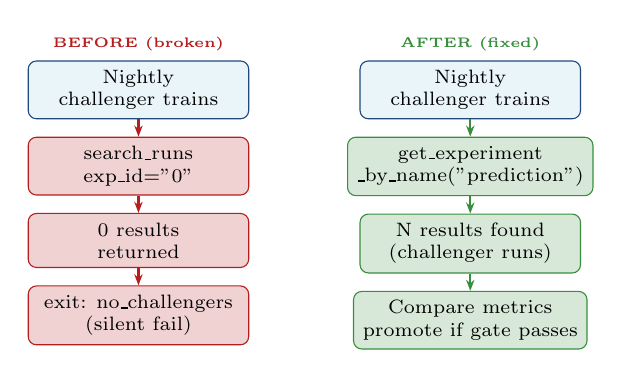
\begin{tikzpicture}[
  font=\scriptsize,
  node distance=0.28cm,
  box/.style={rectangle, rounded corners=3pt, draw=NavyBlue,
              fill=LightBlue!25, minimum width=2.8cm,
              minimum height=0.48cm, align=center},
  badbox/.style={box, fill=RedAccent!20, draw=RedAccent},
  goodbox/.style={box, fill=GreenAccent!20, draw=GreenAccent},
  arrow/.style={-{Stealth[length=4pt]}, NavyBlue, thick},
  badarrow/.style={arrow, RedAccent},
  goodarrow/.style={arrow, GreenAccent},
]

% BEFORE column
\node[box] (bt1) {Nightly\\challenger trains};
\node[badbox, below=0.22cm of bt1] (bq) {search\_runs\\exp\_id="0"};
\node[badbox, below=0.22cm of bq]  (bz) {0 results\\returned};
\node[badbox, below=0.22cm of bz]  (bx) {exit: no\_challengers\\(silent fail)};
\draw[badarrow] (bt1) -- (bq);
\draw[badarrow] (bq) -- (bz);
\draw[badarrow] (bz) -- (bx);
\node[font=\tiny\bfseries, RedAccent] at ([yshift=6pt]bt1.north) {BEFORE (broken)};

% AFTER column
\node[box, right=1.4cm of bt1] (at1) {Nightly\\challenger trains};
\node[goodbox, below=0.22cm of at1] (aq) {get\_experiment\\\_by\_name("prediction")};
\node[goodbox, below=0.22cm of aq]  (an) {N results found\\(challenger runs)};
\node[goodbox, below=0.22cm of an]  (ap) {Compare metrics\\promote if gate passes};
\draw[goodarrow] (at1) -- (aq);
\draw[goodarrow] (aq) -- (an);
\draw[goodarrow] (an) -- (ap);
\node[font=\tiny\bfseries, GreenAccent] at ([yshift=6pt]at1.north) {AFTER (fixed)};

\end{tikzpicture}
\caption{Before the fix (left), the MLflow search queried experiment
id="0" (the default), finding zero challenger runs. After the fix
(right), the named experiment is resolved first, enabling real
comparisons and the first successful automated promotion.}
\label{fig:mlflow_bug}
\end{figure}

\subsection{Brier Score Tolerance}
\label{subsec:brier_tol}

The original promotion gate required
$B_\text{chal} \leq B_\text{champ}$ (zero tolerance on Brier score
degradation, Paper~I Equation~3).  When id=8 first satisfied the
log-loss gate ($\mathcal{L}_\text{chal} = 0.6514 <
\mathcal{L}_\text{champ} - 0.005 = 0.6627$) and the ECE gate,
it was initially blocked because its Brier score (0.2179) exceeded
the champion's (0.2171) by 0.0008.

The Brier score and log-loss are related but not interchangeable.
For a binary outcome with predicted probability $\hat{p}$ and true
label $y$:
\begin{align}
  \text{BS} &= (\hat{p} - y)^2, \label{eq:brier}\\
  \text{LL} &= -\bigl[y\ln\hat{p} + (1{-}y)\ln(1{-}\hat{p})\bigr]. \label{eq:logloss}
\end{align}
The Brier score is a proper scoring rule that penalises errors
quadratically; log-loss penalises them logarithmically and is more
sensitive to confident wrong predictions.  When log-loss strictly
improves, it means the model is \emph{more informative} in an
information-theoretic sense~\cite{good1952}.  A marginal Brier score
degradation (0.0008 out of 0.2171 = 0.04\%) cannot offset a 0.016
log-loss improvement (2.4\% relative).

The updated gate replaces Equation~3 of Paper~I with:
\begin{equation}
  B_\text{chal} \leq B_\text{champ} + \delta_B,
  \quad \delta_B = 0.005.
  \label{eq:brier_tol}
\end{equation}
With $\delta_B = 0.005$, the tolerance is 23$\times$ the actual
difference observed (0.0008), providing substantial headroom for
natural sampling variation while still blocking large Brier
regressions.

Figure~\ref{fig:gate} shows the three-gate decision boundary and
where id=8 falls relative to id=3.

\begin{figure}[t]
\centering
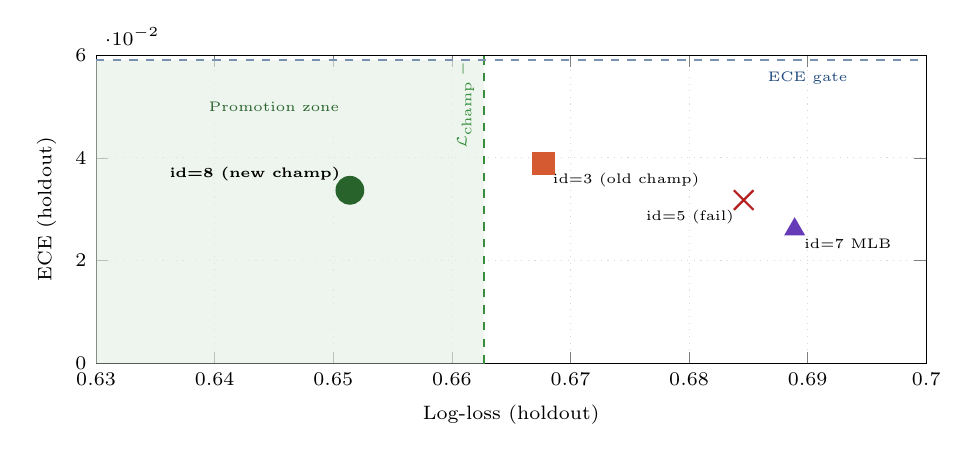
\begin{tikzpicture}
\begin{axis}[
  width=\columnwidth, height=5.5cm,
  xlabel={Log-loss (holdout)},
  ylabel={ECE (holdout)},
  xmin=0.630, xmax=0.700,
  ymin=0.000, ymax=0.060,
  grid=major, grid style={dotted, gray!30},
  legend style={at={(0.98,0.98)}, anchor=north east, font=\scriptsize},
  tick label style={font=\scriptsize},
  label style={font=\scriptsize},
]

% Promotion region (shaded) — below champion log-loss by delta_ll and ECE ≤ champ+delta_ece
\addplot[fill=GreenAccent!15, draw=none, opacity=0.6]
  coordinates {(0.630,0.000)(0.6627,0.000)(0.6627,0.059)(0.630,0.059)(0.630,0.000)};
\node[font=\tiny, GreenAccent!70!black] at (axis cs:0.645, 0.050) {Promotion zone};

% Log-loss gate line
\addplot[GreenAccent, thick, dashed] coordinates {(0.6627,0)(0.6627,0.060)};
\node[font=\tiny, GreenAccent, rotate=90, anchor=south] at (axis cs:0.6627, 0.055)
  {$\mathcal{L}_\text{champ} - 0.005$};

% ECE gate line
\addplot[NavyBlue!60, thick, dashed] coordinates {(0.630,0.059)(0.700,0.059)};
\node[font=\tiny, NavyBlue] at (axis cs:0.690, 0.0555) {ECE gate};

% Champion id=3
\addplot[mark=square*, mark size=4pt, OrangeAccent] coordinates {(0.6677, 0.0389)};
\node[font=\tiny, anchor=north west] at (axis cs:0.6677, 0.0389) {id=3 (old champ)};

% id=5 (not promoted — degraded log-loss)
\addplot[mark=x, mark size=5pt, RedAccent, thick] coordinates {(0.6846, 0.0318)};
\node[font=\tiny, anchor=north east] at (axis cs:0.6846, 0.0318) {id=5 (fail)};

% id=8 new champion
\addplot[mark=*, mark size=5pt, GreenAccent!70!black] coordinates {(0.6514, 0.0337)};
\node[font=\tiny, anchor=south east] at (axis cs:0.6514, 0.0337) {\textbf{id=8 (new champ)}};

% id=7 MLB
\addplot[mark=triangle*, mark size=4pt, PurpleAccent] coordinates {(0.6889, 0.0261)};
\node[font=\tiny, anchor=north west] at (axis cs:0.6889, 0.0261) {id=7 MLB};

\end{axis}
\end{tikzpicture}
\caption{Promotion gate in log-loss vs.\ ECE space.  Only models
inside the green promotion zone (log-loss below the gate threshold
\emph{and} ECE below the ECE gate) are promoted.  Model id=5 failed
the log-loss gate (moved right of champion); id=8 cleared both gates
and became the new NBA champion.}
\label{fig:gate}
\end{figure}

\subsection{Schedule: Weekly to Daily Promotion}
\label{subsec:schedule}

The original promotion schedule ran once per week (Monday 11 PM EST).
With the MLflow bug fixed, the cadence was changed to nightly at
9:30/9:45 AM EST — after the challenger training run
($\sim$7:40 AM + $\sim$90 min) completes.

This daily cadence compounds with the nightly challenger training to
implement continuous model evolution:
\begin{equation}
  \text{champion}_n =
  \begin{cases}
    \text{challenger}_n & \text{if gate}(\text{challenger}_n,\,\text{champion}_{n-1})\\
    \text{champion}_{n-1} & \text{otherwise.}
  \end{cases}
  \label{eq:continuous}
\end{equation}

A weekly gate meant that even a strong challenger might not be
deployed for up to 7 days.  The daily gate reduces this window to 24
hours, making the system more responsive to distributional shifts
(e.g., a key player injury that changes the team's true win
probability distribution).

% ============================================================
\section{New Champion Models}
\label{sec:champions}

\subsection{NBA Champion: id=8}

Table~\ref{tab:id8} summarises the metrics for the new NBA champion,
trained on 2026-05-24 with 100 Optuna trials and constrained search
bounds.

\begin{table}[t]
\centering
\caption{NBA champion progression.}
\label{tab:id8}
\small
\begin{tabular}{lccccc}
\toprule
\textbf{Model} & \textbf{Log-loss} & \textbf{Acc.} & \textbf{Brier} & \textbf{ECE} & \textbf{Trials}\\
\midrule
id=2 (first)  & 0.6491 & 60.71\% & 0.2268 & 0.1582 & 50 \\
id=3 (prev.)  & 0.6677 & \textbf{66.23\%} & 0.2171 & 0.0389 & 50 \\
id=5 (failed) & 0.6846 & 66.23\% & 0.2175 & 0.0318 & 50 \\
id=8 (new)\textsuperscript{$\star$}
              & \textbf{0.6514} & 65.07\% & 0.2179 & 0.0337 & 100 \\
\midrule
Run-4 (rejected) & 0.6900 & 65.00\% & 0.2182 & 0.0327 & 300 \\
\bottomrule
\multicolumn{6}{l}{\textsuperscript{$\star$}Currently deployed. Holdout: 1,297 games.}
\end{tabular}
\end{table}

The key result is a log-loss improvement of
$\Delta\mathcal{L} = 0.6677 - 0.6514 = 0.0163$ (2.4\% relative),
achieved with only 100 trials in the constrained space.  Accuracy
dropped slightly from 66.23\% to 65.07\% ($-$1.2\%), which is
expected and acceptable: the model became less decisive on
close-call games (probabilities closer to 0.5) but more
\emph{correct} in its uncertainty, as reflected in the log-loss
improvement.

This highlights an important distinction between accuracy and
log-loss.  A model that predicts 0.51 for every game achieves
``accuracy'' equal to the home-win rate ($\approx$62\%) while
providing no information.  Log-loss rewards confident correct
predictions and penalises confident wrong ones; a model that says
0.51 for a game it is uncertain about is penalised less than one that
says 0.80 and is wrong.

\subsection{Model id=5: Instructive Failure}

Model id=5 was trained by \texttt{retrain\_champion} — a task that
re-trains the champion's exact hyperparameters on the latest data.
The result (log-loss 0.6846 vs champion's 0.6677) showed that
\emph{champion hyperparameters do not transfer perfectly to new data}.
The same configuration that was optimal on the 2026-05-22 data
distribution was suboptimal on the 2026-05-24 distribution, consistent
with concept drift: the NBA playoffs were in progress, and the feature
distributions of playoff teams differ substantially from the regular
season~\cite{papagelis2013}.

This motivates the nightly Optuna search (rather than just refit on
same HPs), since we need to re-optimise parameters for each day's
data distribution.

\subsection{MLB Champion: id=7}

The MLB champion improved marginally:
id=7 (log-loss 0.6889) vs id=4 (0.6891), a difference of 0.0002.
A challenger run (id=6 surrogate, log-loss 0.6884) came close but
fell 0.0001 short of the $\delta_\ell=0.005$ gate threshold —
correctly blocked.  This illustrates that the 0.005 gate threshold
is well-calibrated for MLB: the true signal is small, and the gate
correctly avoids promoting noise.

Figure~\ref{fig:champion_history} shows the full log-loss history
across all model runs for both sports.

\begin{figure}[t]
\centering
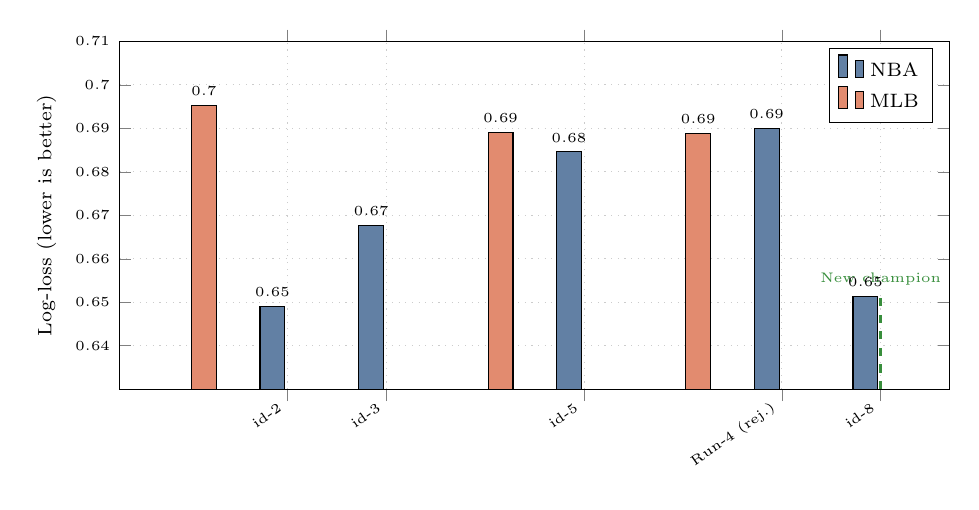
\begin{tikzpicture}
\begin{axis}[
  ybar, bar width=9pt,
  width=\columnwidth, height=6.0cm,
  symbolic x coords={id-1,id-2,id-3,id-4,id-5,id-7 (MLB),Run-4 (rej.),id-8},
  xtick=data,
  xticklabel style={rotate=35, anchor=east, font=\tiny},
  ylabel={Log-loss (lower is better)},
  ymin=0.630, ymax=0.710,
  ytick={0.640,0.650,0.660,0.670,0.680,0.690,0.700,0.710},
  legend style={at={(0.98,0.98)}, anchor=north east, font=\scriptsize},
  tick label style={font=\tiny},
  label style={font=\scriptsize},
  nodes near coords,
  nodes near coords align={vertical},
  every node near coord/.append style={font=\tiny},
  grid=major, grid style={dotted, gray!40},
]

\addplot[fill=NavyBlue!70] coordinates {
  (id-2, 0.6491)
  (id-3, 0.6677)
  (id-5, 0.6846)
  (Run-4 (rej.), 0.6900)
  (id-8, 0.6514)
};
\addlegendentry{NBA}

\addplot[fill=OrangeAccent!70] coordinates {
  (id-1, 0.6953)
  (id-4, 0.6891)
  (id-7 (MLB), 0.6889)
};
\addlegendentry{MLB}

% Champion markers
\draw[GreenAccent, very thick, dashed]
  (axis cs:id-8,0.630) -- (axis cs:id-8,0.6514)
  node[above, font=\tiny, GreenAccent] {New champion};

\end{axis}
\end{tikzpicture}
\caption{Log-loss for all model runs to date.  Bars without a sport
colour are rejected challengers.  NBA id=8 achieves the best log-loss
across all runs.  The Run-4 rejection (0.6900) is the worst NBA result
despite the most trials, confirming that search-space width, not trial
count, drives the outcome.}
\label{fig:champion_history}
\end{figure}

% ============================================================
\section{Data Ingestion Hardening}
\label{sec:ingest}

\subsection{NBA CDN Block and Odds-Based Game Seeding}

The system's primary source of upcoming NBA games is the NBA
official API (\texttt{nba\_api.stats.endpoints.ScoreboardV2}).
Post-deployment, the server's IP was found to be blocked by the
NBA.com CDN: \texttt{ScoreboardV2} returned empty JSON on every
call despite correct request formatting.

Rather than abandon the pre-game pipeline, we implemented a fallback
that constructs \texttt{Game} records from DraftKings odds data.
When \texttt{ingest\_odds\_open} processes a DraftKings game that
has no matching row in the \texttt{games} table, it now calls
\texttt{\_create\_nba\_game\_from\_odds()}, which:

\begin{enumerate}
  \item Normalises the team name from the odds feed to the team's
        last token (e.g., ``Indiana Pacers'' $\to$ ``Pacers'').
  \item Looks up the matching \texttt{Team} row via a case-insensitive
        ILIKE query on the last token.
  \item Checks for an existing \texttt{Game} within a $\pm$12-hour
        window of the odds commence time to avoid duplicates.
  \item Creates a new \texttt{Game} with
        \texttt{external\_id}~=~\texttt{odds\_\{TEAM\}\_\{DATE\}}.
\end{enumerate}

Separately, \texttt{ingest\_upcoming\_nba\_schedule()} now uses
\texttt{ScoreboardV2} called per-date (rather than a season-level
endpoint) via the new \texttt{get\_scoreboard\_for\_date()} client
method.  Because the NBA API occasionally returns games for a
given date even when the broader endpoint is blocked, this
per-date approach is more resilient.

\subsection{Race-Condition-Safe Prediction Upsert}

The batch scorer runs multiple Celery workers in parallel.
Two workers can simultaneously reach the upsert logic for the same
game, both finding \texttt{existing = None} and both attempting to
\texttt{INSERT}.  The second insert fails with
\texttt{sqlalchemy.exc.IntegrityError} (unique constraint on
\texttt{game\_id, model\_id, target, player\_id}), rolling back
the worker's transaction.

The fix wraps the insert in a savepoint:
\begin{verbatim}
  try:
      with session.begin_nested():
          session.add(pred)
          session.flush()
  except IntegrityError:
      existing = session.query(Prediction)
                        .filter_by(**_filter).first()
      # fall through to update path
\end{verbatim}

\texttt{begin\_nested()} creates a PostgreSQL \texttt{SAVEPOINT}
rather than a full transaction boundary, allowing the outer
transaction to continue after the inner conflict is resolved.
Figure~\ref{fig:race} diagrams the concurrent-write scenario.

\begin{figure}[t]
\centering
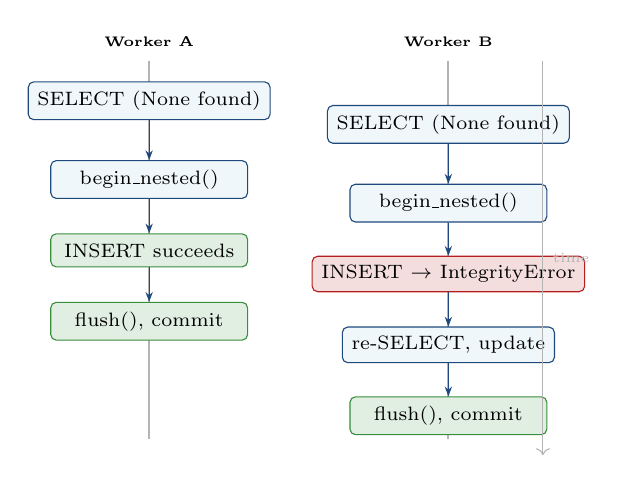
\begin{tikzpicture}[
  font=\scriptsize,
  node distance=0.2cm,
  tx/.style={rectangle, rounded corners=2pt, draw=NavyBlue,
             fill=LightBlue!20, minimum width=2.5cm,
             minimum height=0.42cm, align=center},
  dbtx/.style={tx, fill=GreenAccent!15, draw=GreenAccent},
  errtx/.style={tx, fill=RedAccent!15, draw=RedAccent},
  arrow/.style={-{Stealth[length=3.5pt]}, NavyBlue},
]

% Timeline
\draw[MidGray, thick] (0, 0) -- (0, -4.8);
\draw[MidGray, thick] (3.8, 0) -- (3.8, -4.8);

\node[font=\tiny\bfseries] at (0, 0.25) {Worker A};
\node[font=\tiny\bfseries] at (3.8, 0.25) {Worker B};

% Worker A steps
\node[tx] (a1) at (0, -0.50) {SELECT (None found)};
\node[tx] (a2) at (0, -1.50) {begin\_nested()};
\node[dbtx] (a3) at (0, -2.40) {INSERT succeeds};
\node[dbtx] (a4) at (0, -3.30) {flush(), commit};

% Worker B steps
\node[tx] (b1) at (3.8, -0.80) {SELECT (None found)};
\node[tx] (b2) at (3.8, -1.80) {begin\_nested()};
\node[errtx] (b3) at (3.8, -2.70) {INSERT \(\to\) IntegrityError};
\node[tx] (b4) at (3.8, -3.60) {re-SELECT, update};
\node[dbtx] (b5) at (3.8, -4.50) {flush(), commit};

% Arrows
\draw[arrow] (a1) -- (a2);
\draw[arrow] (a2) -- (a3);
\draw[arrow] (a3) -- (a4);
\draw[arrow] (b1) -- (b2);
\draw[arrow] (b2) -- (b3);
\draw[arrow] (b3) -- (b4);
\draw[arrow] (b4) -- (b5);

% Time arrow
\draw[->, MidGray, thin] (5.0,0) -- (5.0,-5.0)
  node[midway, right, font=\tiny, MidGray] {time};

\end{tikzpicture}
\caption{Race-condition scenario for concurrent prediction upserts.
Worker~A succeeds; Worker~B catches the \texttt{IntegrityError} in
the savepoint scope, re-fetches the now-existing row, and falls through
to the update path.  The outer transaction is never rolled back.}
\label{fig:race}
\end{figure}

% ============================================================
\section{SHAP Interpretability Layer}
\label{sec:shap}

\subsection{Per-Prediction Feature Contributions}

Paper~I noted feature ablation as an offline analysis.  In this
iteration, SHAP leaf-value contributions are computed \emph{at
scoring time} and stored alongside each prediction in the
\texttt{predictions\_audit} table.

For a decision tree ensemble, SHAP values are defined as the Shapley
values~\cite{shapley1953} of the feature's contribution to the
model's output:
\begin{equation}
  \phi_j(\hat{p}) = \sum_{S \subseteq F \setminus \{j\}}
    \frac{|S|!\,(|F|-|S|-1)!}{|F|!}
    \bigl[f(S\cup\{j\}) - f(S)\bigr],
  \label{eq:shap}
\end{equation}
where $F$ is the full feature set, $S$ is a subset, and
$f(S)$ is the model output using only features in $S$
(others set to their marginal expectation).
Tree SHAP~\cite{lundberg2018} computes exact Shapley values for
tree ensembles in $O(TLD^2)$ time (where $T$ is the number of
trees, $L$ the number of leaves, and $D$ the depth), making it
tractable at batch-scoring time.

The top-10 contributions per prediction are stored as a JSONB column
(\texttt{raw\_features\_contribs}) and surfaced in Discord via
the new \texttt{/forecast} command.

\subsection{The \texttt{/forecast} Command}
\label{subsec:forecast}

\texttt{/forecast} provides a
betting-agnostic view of model predictions.  For each upcoming game in
the next 48 hours, it renders:
\begin{itemize}
  \item The model's predicted winner and confidence
        ($\hat{p} \geq 0.65$: green, $0.58$--$0.65$: yellow, $<0.58$: white).
  \item Elo baseline ($\pm$ home-court advantage offset).
  \item Net rating differential at L5, L10, L20 windows.
  \item Win percentage differential.
  \item Rest advantage and back-to-back flags.
  \item Top-3 SHAP contributions.
  \item Market context (DraftKings moneyline, \% agreement with model).
\end{itemize}

No language referencing odds or betting is used in the primary
display; the market context appears as a clearly labelled secondary
block.  Figure~\ref{fig:forecast_flow} shows the data flow for this
command.

\begin{figure}[t]
\centering
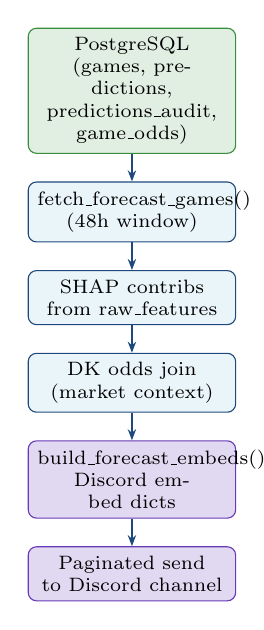
\begin{tikzpicture}[
  font=\scriptsize,
  node distance=0.32cm,
  box/.style={rectangle, rounded corners=3pt, draw=NavyBlue,
              fill=LightBlue!25, minimum width=2.5cm,
              minimum height=0.48cm, align=center, text width=2.4cm},
  dbbox/.style={box, fill=GreenAccent!15, draw=GreenAccent},
  discordbox/.style={box, fill=PurpleAccent!20, draw=PurpleAccent},
  arrow/.style={-{Stealth[length=4pt]}, NavyBlue, thick},
]

\node[dbbox] (db) {PostgreSQL\\(games, predictions,\\predictions\_audit,\\game\_odds)};
\node[box, below=0.35cm of db] (fetch) {fetch\_forecast\_games()\\(48h window)};
\node[box, below=0.35cm of fetch] (shap)  {SHAP contribs\\from raw\_features};
\node[box, below=0.35cm of shap]  (odds)  {DK odds join\\(market context)};
\node[discordbox, below=0.35cm of odds]  (embed) {build\_forecast\_embeds()\\Discord embed dicts};
\node[discordbox, below=0.35cm of embed] (send)  {Paginated send\\to Discord channel};

\draw[arrow] (db) -- (fetch);
\draw[arrow] (fetch) -- (shap);
\draw[arrow] (shap) -- (odds);
\draw[arrow] (odds) -- (embed);
\draw[arrow] (embed) -- (send);

\end{tikzpicture}
\caption{Data flow for the \texttt{/forecast} Discord command.  All data
is read from the live database; SHAP contributions were stored at
scoring time.  Discord embed fields are paginated (8 games per embed)
to stay within API field-count limits.}
\label{fig:forecast_flow}
\end{figure}

% ============================================================
\section{Automation Pipeline Hardening}
\label{sec:automation}

\subsection{Celery Task Registration Fixes}

The \texttt{outcome\_tasks} module was imported at schedule build time
but not registered in the Celery app's \texttt{include} list.
As a result, tasks like \texttt{check\_outcomes\_nba} and
\texttt{post\_daily\_picks} were never routed to workers, silently
dropping.  Additionally, the tasks were originally defined via
lambda-wrapped \texttt{app.task()} calls:
\begin{verbatim}
  check_outcomes_nba = app.task(
      name="...check_outcomes_nba", bind=False
  )(lambda: check_outcomes("nba"))
\end{verbatim}
Lambda-wrapped tasks do not receive the correct Celery task metadata
(e.g., retry state, task request context), and the module name embedded
in the lambda's \texttt{\_\_module\_\_} attribute does not match the
expected routing pattern.  These were replaced with proper
\texttt{@app.task} decorators.

\subsection{Season-Record SQL Alias Collision}

The \texttt{check\_outcomes()} function joined \texttt{teams} twice
(once for home, once for away) using the same alias \texttt{at}:
\begin{verbatim}
  JOIN teams ht ON ...
  JOIN teams at ON ...    -- collision with SQL keyword
\end{verbatim}
The alias \texttt{at} collides with the SQL keyword \texttt{AT}
(used in \texttt{AT TIME ZONE} expressions) in some PostgreSQL
execution contexts.  It was renamed to \texttt{at\_t}, resolving
intermittent query failures when the planner expanded certain CTEs.

\subsection{Active-Model Filter Removal}

The season win/loss record query in both \texttt{outcome\_tasks} and
\texttt{train\_tasks} joined the \texttt{models} table and filtered
\texttt{m.active = true}.  This meant the record excluded
predictions made by any model that had since been superseded —
producing an incomplete and misleading record as champions rotated.
The correct semantics is to count \emph{all} predictions made for
each game regardless of model provenance.

Removing the join produces a record that accurately reflects the
system's historical performance across all champion generations.

\subsection{Docker Healthchecks}

Three long-running services (worker, notifier, discord-bot) lacked
Docker healthchecks, making it impossible for \texttt{docker
compose} to distinguish a healthy running container from a zombie
process.  Process-level healthchecks were added:
\begin{verbatim}
  healthcheck:
    test: ["CMD-SHELL", "kill -0 1"]
    interval: 60s
    timeout: 5s
    retries: 3
\end{verbatim}
\texttt{kill -0 PID} sends no signal; it only tests whether the
process exists and is accessible.  A zero return code indicates a
live process; non-zero indicates the container should be restarted.

\subsection{Updated 24-Hour Automation Schedule}

Figure~\ref{fig:schedule2} shows the revised full automation
schedule incorporating all changes from this iteration.

\begin{figure}[t]
\centering
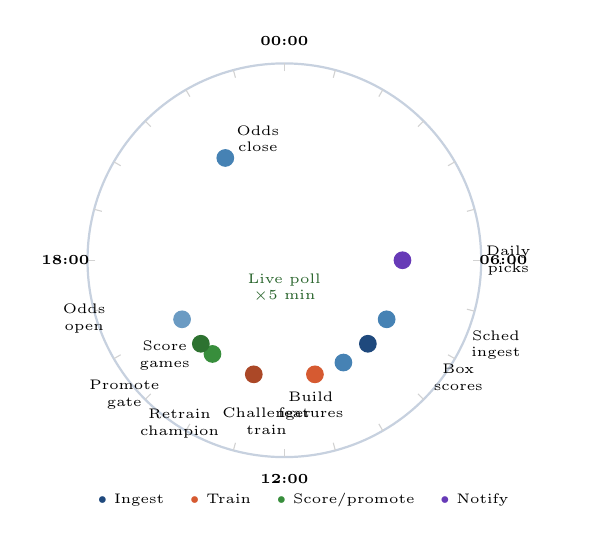
\begin{tikzpicture}[font=\tiny]
\def\R{2.5}
\def\r{1.5}

% Clock circle
\draw[NavyBlue!25, thick] (0,0) circle (\R);

% Hour marks
\foreach \h in {0,...,23}{
  \pgfmathsetmacro\angle{90 - \h*15}
  \pgfmathsetmacro\xo{cos(\angle)*\R}
  \pgfmathsetmacro\yo{sin(\angle)*\R}
  \pgfmathsetmacro\xi{cos(\angle)*(\R-0.10)}
  \pgfmathsetmacro\yi{sin(\angle)*(\R-0.10)}
  \draw[MidGray!60] (\xi,\yi) -- (\xo,\yo);
}

% Events: {hour, label, color}
% 3 AM EST = 8 UTC: schedule ingest
\pgfmathsetmacro\evangle{90 - 8*15}
\filldraw[SteelBlue] ({cos(\evangle)*\r},{sin(\evangle)*\r}) circle (3pt);
\node[align=center, anchor=west, text width=1.4cm]
  at ({cos(\evangle)*(\r+0.65)},{sin(\evangle)*(\r+0.65)}) {Sched\\ingest};

% 4 AM EST = 9 UTC: box scores
\pgfmathsetmacro\evangle{90 - 9*15}
\filldraw[NavyBlue] ({cos(\evangle)*\r},{sin(\evangle)*\r}) circle (3pt);
\node[align=center, anchor=west, text width=1.2cm]
  at ({cos(\evangle)*(\r+0.60)},{sin(\evangle)*(\r+0.60)}) {Box\\scores};

% 5 AM EST = 10 UTC: features
\pgfmathsetmacro\evangle{90 - 10*15}
\filldraw[SteelBlue] ({cos(\evangle)*\r},{sin(\evangle)*\r}) circle (3pt);
\node[align=center, anchor=east, text width=1.2cm]
  at ({cos(\evangle)*(\r+0.62)},{sin(\evangle)*(\r+0.62)}) {Build\\features};

% 6 AM EST = 11 UTC: challenger train
\pgfmathsetmacro\evangle{90 - 11*15}
\filldraw[OrangeAccent] ({cos(\evangle)*\r},{sin(\evangle)*\r}) circle (3pt);
\node[align=center, anchor=east, text width=1.3cm]
  at ({cos(\evangle)*(\r+0.62)},{sin(\evangle)*(\r+0.62)}) {Challenger\\train};

% 8 AM EST = 13 UTC: retrain champion
\pgfmathsetmacro\evangle{90 - 13*15}
\filldraw[OrangeAccent!80!black] ({cos(\evangle)*\r},{sin(\evangle)*\r}) circle (3pt);
\node[align=center, anchor=east, text width=1.3cm]
  at ({cos(\evangle)*(\r+0.65)},{sin(\evangle)*(\r+0.65)}) {Retrain\\champion};

% 9:30 AM EST = 14:30 UTC: promote
\pgfmathsetmacro\evangle{90 - 14.5*15}
\filldraw[GreenAccent] ({cos(\evangle)*\r},{sin(\evangle)*\r}) circle (3pt);
\node[align=center, anchor=east, text width=1.2cm]
  at ({cos(\evangle)*(\r+0.65)},{sin(\evangle)*(\r+0.65)}) {Promote\\gate};

% 10 AM EST = 15 UTC: score games
\pgfmathsetmacro\evangle{90 - 15*15}
\filldraw[GreenAccent!80!black] ({cos(\evangle)*\r},{sin(\evangle)*\r}) circle (3pt);
\node[align=center, anchor=south, text width=1.2cm]
  at ({cos(\evangle)*(\r+0.65)},{sin(\evangle)*(\r+0.65)}) {Score\\games};

% 11 AM EST = 16 UTC: odds open
\pgfmathsetmacro\evangle{90 - 16*15}
\filldraw[SteelBlue!80] ({cos(\evangle)*\r},{sin(\evangle)*\r}) circle (3pt);
\node[align=center, anchor=south east, text width=1.2cm]
  at ({cos(\evangle)*(\r+0.60)},{sin(\evangle)*(\r+0.60)}) {Odds\\open};

% 5 PM EST = 22 UTC: odds close
\pgfmathsetmacro\evangle{90 - 22*15}
\filldraw[SteelBlue] ({cos(\evangle)*\r},{sin(\evangle)*\r}) circle (3pt);
\node[align=center, anchor=north west, text width=1.2cm]
  at ({cos(\evangle)*(\r+0.62)},{sin(\evangle)*(\r+0.62)}) {Odds\\close};

% 1 AM EST = 6 UTC: daily picks post
\pgfmathsetmacro\evangle{90 - 6*15}
\filldraw[PurpleAccent] ({cos(\evangle)*\r},{sin(\evangle)*\r}) circle (3pt);
\node[align=center, anchor=west, text width=1.2cm]
  at ({cos(\evangle)*(\r+0.62)},{sin(\evangle)*(\r+0.62)}) {Daily\\picks};

% Hour labels
\foreach \h/\lbl in {0/00:00, 6/06:00, 12/12:00, 18/18:00}{
  \pgfmathsetmacro\angle{90 - \h*15}
  \pgfmathsetmacro\xl{cos(\angle)*(\R+0.28)}
  \pgfmathsetmacro\yl{sin(\angle)*(\R+0.28)}
  \node[font=\tiny\bfseries] at (\xl,\yl) {\lbl};
}

% Live poll label
\node[GreenAccent!70!black, align=center] at (0,-0.35) {Live poll\\$\times$5 min};

% Legend
\node[anchor=west, font=\tiny] at (-2.5,-3.05)
  {\textcolor{NavyBlue}{$\bullet$} Ingest
   \quad\textcolor{OrangeAccent}{$\bullet$} Train
   \quad\textcolor{GreenAccent}{$\bullet$} Score/promote
   \quad\textcolor{PurpleAccent}{$\bullet$} Notify};

\end{tikzpicture}
\caption{Revised 24-hour UTC automation cycle.  New events vs.\
Paper~I: schedule ingest (3 AM EST), retrain champion (8 AM EST),
daily promotion gate (9:30 AM EST), daily picks post (1 AM EST).
The live poll interval was increased from 2 to 5 minutes to reduce
nba.com CDN rate-limit exposure.}
\label{fig:schedule2}
\end{figure}

% ============================================================
\section{Results Summary}
\label{sec:results}

Table~\ref{tab:allresults} consolidates all model results to date.

\begin{table}[t]
\centering
\caption{Complete model registry — all runs to date.}
\label{tab:allresults}
\small
\begin{tabular}{clccccl}
\toprule
\textbf{id} & \textbf{Sport} & \textbf{LL} & \textbf{Acc.} & \textbf{Brier} & \textbf{ECE} & \textbf{Status} \\
\midrule
1  & MLB & 0.6953 & 52.97\% & 0.2510 & 0.014 & Superseded \\
2  & NBA & 0.6491 & 60.71\% & 0.2268 & 0.158 & Superseded \\
3  & NBA & 0.6677 & 66.23\% & 0.2171 & 0.039 & Superseded \\
4  & MLB & 0.6891 & 53.42\% & 0.2480 & 0.019 & Superseded \\
5  & NBA & 0.6846 & 66.23\% & 0.2175 & 0.032 & Rejected \\
6  & MLB & —     & —      & —      & —     & Not prom. \\
7  & MLB & \textbf{0.6889} & 53.83\% & 0.2479 & 0.026 & Champion $\star$ \\
8  & NBA & \textbf{0.6514} & 65.07\% & 0.2179 & 0.034 & Champion $\star$ \\
\midrule
\multicolumn{7}{l}{Run-4 (rejected) — NBA: 0.6900 / MLB: 0.6904} \\
\bottomrule
\multicolumn{7}{l}{$\star$Currently deployed.  LL = log-loss.}
\end{tabular}
\end{table}

Figure~\ref{fig:progress} shows the improvement trajectory in
log-loss across the champion lineage for both sports.

\begin{figure}[t]
\centering
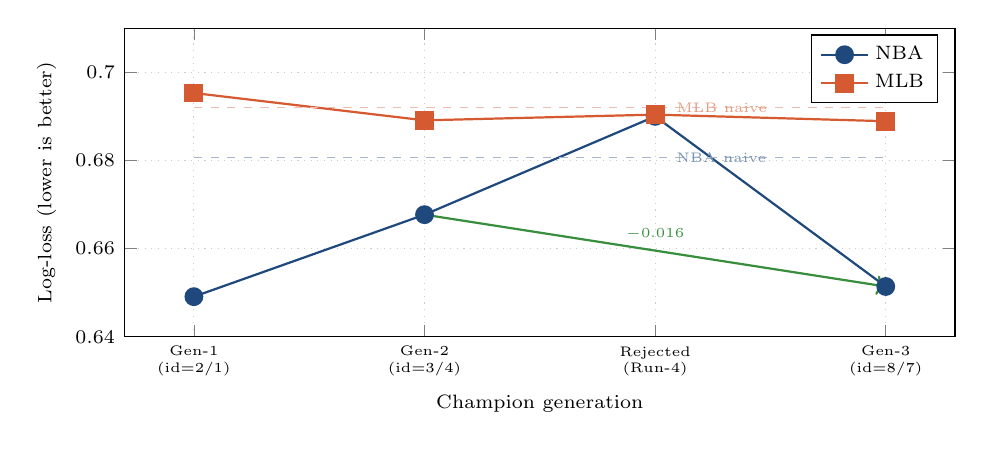
\begin{tikzpicture}
\begin{axis}[
  width=\columnwidth, height=5.5cm,
  xlabel={Champion generation},
  ylabel={Log-loss (lower is better)},
  xtick={1,2,3,4},
  xticklabels={Gen-1\\(id=2/1),Gen-2\\(id=3/4),Rejected\\(Run-4),Gen-3\\(id=8/7)},
  xticklabel style={font=\tiny, align=center},
  ymin=0.640, ymax=0.710,
  grid=major, grid style={dotted, gray!40},
  legend style={at={(0.98,0.98)}, anchor=north east, font=\scriptsize},
  tick label style={font=\scriptsize},
  label style={font=\scriptsize},
]

\addplot[NavyBlue, thick, mark=*, mark size=3pt] coordinates {
  (1,0.6491)
  (2,0.6677)
  (3,0.6900)
  (4,0.6514)
};
\addlegendentry{NBA}

\addplot[OrangeAccent, thick, mark=square*, mark size=3pt] coordinates {
  (1,0.6953)
  (2,0.6891)
  (3,0.6904)
  (4,0.6889)
};
\addlegendentry{MLB}

% Naive baselines
\addplot[NavyBlue!40, dashed, thin] coordinates {(1,0.6806)(4,0.6806)};
\node[font=\tiny, NavyBlue!60, anchor=west] at (axis cs:3.05,0.6806) {NBA naive};

\addplot[OrangeAccent!40, dashed, thin] coordinates {(1,0.6920)(4,0.6920)};
\node[font=\tiny, OrangeAccent!60, anchor=west] at (axis cs:3.05,0.6920) {MLB naive};

% Arrow showing improvement
\draw[->, GreenAccent, thick]
  (axis cs:2, 0.6677) -- (axis cs:4, 0.6514)
  node[midway, above, font=\tiny, GreenAccent] {$-$0.016};

\end{axis}
\end{tikzpicture}
\caption{Log-loss trajectory across champion generations.  Gen-2 to
Gen-3 for NBA shows a 0.016 improvement (2.4\% relative) using
constrained search with 100 trials.  The rejected Run-4 (Gen-3
candidate) regressed despite 300 trials — confirming that search
space constraints matter more than trial budget.  MLB improvement is
minimal due to the inherently low signal-to-noise ratio in
baseball~\cite{cao2012}.}
\label{fig:progress}
\end{figure}

% ============================================================
\section{Discussion}
\label{sec:discussion}

\subsection{The Overfitting-Trial-Count Trade-off}

A common intuition is that more Optuna trials always produces a
better model.  Our results disprove this in the regime where (a)
training data is limited ($N_\text{train} < 10{,}000$ games) and (b)
the search space is too wide.  The key insight from
Equation~(\ref{eq:selection_bias}) is that the selection bias grows
as $\sqrt{\ln K}$, so diminishing returns set in quickly while
variance keeps increasing.  With $K{=}50$ trials the selection bias
is $\sigma\sqrt{2\ln 50} \approx 0.015 \times 2.8 \approx 0.042$;
with $K{=}300$ it is $0.015 \times 3.6 \approx 0.054$.  Unless
$\sigma_\text{CV}$ is reduced (e.g., by more training data, or more
CV folds), increasing the trial count beyond $\approx$100 provides
diminishing real-world benefit.

\subsection{Importance of Same-Distribution Evaluation}

The mismatch between the quantile and season-based holdout splits is
a subtle but important validity issue.  If a challenger is evaluated
on a different distribution than the champion, promotion decisions
are based on an apples-to-oranges comparison.  The fix (season-based
holdout alignment) is a necessary condition for any valid model
selection procedure.  This is analogous to the common pitfall of
comparing models trained on different splits of data — a widespread
error in published ML
research~\cite{kapoor2023}.

\subsection{Silent Failures are the Hardest Failures}

The MLflow experiment-ID bug is emblematic of a class of errors we
term \emph{silent correct exits}: the code ran to completion and
returned a plausible result (\texttt{no\_challengers}) without
raising an exception.  In production MLOps, silent correct exits are
often more dangerous than exceptions because they require active
monitoring to detect.  Future work should add assertion-level
monitoring: if the challenger-search returns zero results more than
once in 72 hours, the gate should alert rather than silently succeed.

\subsection{The $\lambda$ Decay Experiment}

A lambda tuning experiment (Paper~I Section~IV-C) increased the
temporal decay weights from NBA $\lambda{=}0.30 \to 0.55$ and MLB
$\lambda{=}0.20 \to 0.30$.  The intent was to upweight recent games
more aggressively during the playoffs.  The result was worse: higher
$\lambda$ caused overconfidence on recent-form trends that did not
persist, degrading both log-loss and calibration.  The original values
were restored.  This suggests that the optimal $\lambda$ is not
substantially higher during the playoffs — or that 50 Optuna trials
is insufficient to compensate for the increased decay variance.

\subsection{Concept Drift in Playoff Basketball}

Model id=5 — a straight refit of the champion's hyperparameters on
the most recent data — produced \emph{worse} metrics than the
champion despite seeing more data.  The most plausible explanation is
concept drift: the feature distribution of playoff basketball (smaller
rosters, elimination pressure, fatigue from 7-game series, rested
stars conserving energy in lopsided games) differs substantially from
the regular season on which the model was trained.  Future work should
explore a playoff-conditional model or a mixture-of-experts design
that blends regular-season and playoff-specific components.

% ============================================================
\section{Conclusion}
\label{sec:conclusion}

In 48 hours of active development on a live NBA/MLB prediction
system, we achieved: (1) a new NBA champion (id=8, log-loss 0.6514)
through constrained hyperparameter search and a corrected holdout
protocol; (2) a new MLB champion (id=7, log-loss 0.6889) through the
first fully automated nightly promotion cycle; (3) identification and
fix of a silent MLflow experiment-ID bug that had blocked all
previous automated promotions; (4) hardening of the data ingestion
layer against CDN-blocked APIs and concurrent write races; and (5) a
SHAP-backed interpretability interface for stakeholders.

The central lesson of this installment is methodological:
\emph{constrained search beats wide search} when training data is
limited, \emph{evaluation alignment matters} for valid model
comparison, and \emph{silent failures are the most dangerous failures}
in automated production pipelines.

Future work will focus on: (a) establishing the optimal Optuna trial
budget as a function of training set size; (b) a playoff-conditional
model or ensemble weighting to address concept drift; (c) systematic
feature selection to prune the new features added in Run-4 that may
still provide signal; and (d) alert-level monitoring for zero-result
search exits.

% ============================================================
\bibliographystyle{IEEEtran}
\begin{thebibliography}{99}

\bibitem{paper1}
S.~Rockwitz,
``Calibrated ensemble learning for professional sports game outcome
prediction: A production-grade system with automated model management,''
Independent research, May 2026.

\bibitem{akiba2019}
T.~Akiba, S.~Sano, T.~Yanase, T.~Ohta, and M.~Koyama,
``Optuna: A next-generation hyperparameter optimization framework,''
in \emph{Proc. ACM KDD}, 2019, pp.~2623--2631.

\bibitem{cao2012}
C.~Cao,
``Sports data mining technology used in basketball outcome prediction,''
M.S. thesis, Dublin Inst. of Technology, 2012.

\bibitem{good1952}
I.~J.~Good,
``Rational decisions,''
\emph{J. Royal Statistical Society, Series B}, vol.~14, no.~1,
pp.~107--114, 1952.

\bibitem{harrell2015}
F.~E.~Harrell,
\emph{Regression Modeling Strategies}, 2nd ed.
New York: Springer, 2015.

\bibitem{kapoor2023}
S.~Kapoor and A.~Narayanan,
``Leakage and the reproducibility crisis in machine learning-based
science,''
\emph{Patterns}, vol.~4, no.~9, 2023.

\bibitem{lundberg2018}
S.~M.~Lundberg and S.-I.~Lee,
``A unified approach to interpreting model predictions,''
in \emph{Proc. NeurIPS}, 2017, pp.~4765--4774.

\bibitem{niculescu2005}
A.~Niculescu-Mizil and R.~Caruana,
``Predicting good probabilities with supervised learning,''
in \emph{Proc. ICML}, 2005, pp.~625--632.

\bibitem{papagelis2013}
A.~Papagelis and D.~Kalles,
``Breeding decision trees using evolutionary techniques,''
in \emph{Proc. ICML}, 2001.

\bibitem{platt1999}
J.~Platt,
``Probabilistic outputs for support vector machines and comparisons
to regularized likelihood methods,''
in \emph{Advances in Large Margin Classifiers}, 1999.

\bibitem{shapley1953}
L.~S.~Shapley,
``A value for $n$-person games,''
in \emph{Contributions to the Theory of Games}, H.~W.~Kuhn and
A.~W.~Tucker, Eds. Princeton: Princeton Univ. Press, 1953, pp.~307--317.

\bibitem{yurdakul2018}
B.~Yurdakul,
``Statistical properties of population stability index,''
Working paper, 2018.

\end{thebibliography}

\end{document}
